\section{Zusammenfassung und Diskussion}

In Versuch 222 setzten wir uns mit dem Heißluft- bzw. Stirlingmotor auseinander. Dieser wurde im Jahr 1816 von Robert Stirling zum Patent angemeldet. Die Funktionsweise des Heißluftmotors basiert auf einem thermodynamischen Kreisprozess aus abwechselnden isothermen und isochoren Zustandsänderungen, welchen wir im Versuch quantitativ untersuchten.

Im ersten Versuchsteil wurde der Heißluftmotor zunächst nicht als Motor im klassischen Sinne verwendet. Stattdessen trieben wir diesen mit einem externen Motor an, führten also mechanische Arbeit von außen zu. Hierdurch ist es möglich, den eigentlichen Kreisprozess des Motors umzukehren und ihn als Kältemaschine oder auch Wärmepumpe, zur Abkühlung bzw. Aufheizung eines Reservoirs zu verwenden. Die erste Aufgabe war es, die Kälteleistung und Wirkungsgrad der Kältemaschine zu berechnen, sowie die Energiebilanz im System zu untersuchen. Hierzu montierten wir am Zylinder der Kältemaschine eine Heizwendel, mit welcher die entzogene Wärme kompensiert wurde. Anhand der Heizleistung berechneten wir dann die Kälteleistung pro Motorumdrehung zu
\begin{align*}
  Q_2 = (4.21 \pm 0.05)\si{\joule},
\end{align*}
was in Relation zur zugeführten mechanischen Arbeit einem Wirkungsgrad von
\begin{align*}
  \eta = 0.440 \pm 0.022
\end{align*}
entsprach. Eine Untersuchung der Energiebilanz zeigte auf, dass dem System im Prozess eine Energie von
\begin{align*}
  \Delta Q = (8.1 \pm 0.7)\si{\joule}
\end{align*}
verloren geht. Diese großen Energieverluste könnten sich auf Wärmeverluste durch unzureichende Isolation, mechanische Reibung, ineffiziente Energieübertragung und Verluste im Kühlkreislauf zurückführen lassen. Zusätzlich könnten Messfehler oder Unsicherheiten sowie das nicht-ideale Verhalten des realen Stirlingprozesses, dies zeigt sich durch die abgerundeten Isochoren, eine Rolle spielen. Auch Effizienzverluste des Elektromotors bei der Umwandlung von elektrischer Energie zu mechanischer Arbeit können Gründe für die Abweichungen sein.

Für den zweiten Versuchsteil trieben wir den Heißluftmotor weiterhin extern an. Anstelle der Heizwendel montierten wir nun ein Reagenzglas mit Wasser am Motor. Wir betrieben diesen zunächst erneut als Kältemaschine, um das Wasser auf etwa $-30\si{\celsius}$ herunterzukühlen und anschließend als Wärmepumpe um das Wasser wieder aufzuheizen, bis es in etwa $100\si{\celsius}$ erreichte. Über den kompletten Vorgang hinweg zeichneten wir die Wassertemperatur auf. Eine detaillierte Interpretation des Temperaturverlaufs ist im entsprechenden Abschnitt der Ausarbeitung zu finden. Abbildung \abbref{fig:tempverlauf_unter0} zeigt noch einmal den interessantesten Teil des Temperaturverlaufs um und unter der $0\si{\celsius}$-Marke.

\begin{figure}[H]
  \centering
  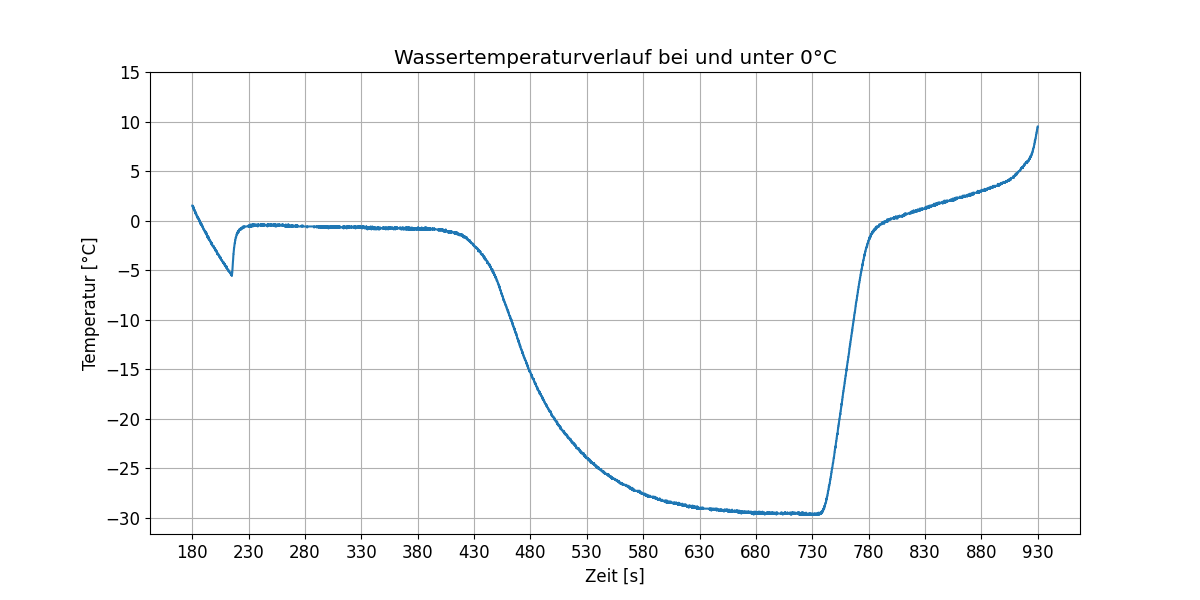
\includegraphics[width=.9\textwidth]{files/tempverlauf_unter0.png}
  \caption{Wassertemperaturverlauf beim Betrieb als Kältemaschine und Wärmepumpe für etwa $1 \si{\milli\liter}$ Wasser um und unter $0\si{\celsius}$.}
  \label{fig:tempverlauf_unter0}
\end{figure}

Besonderes Augenmerk legten wir hierbei auf den Plateaubereich, der sich ab etwa Sekunde $230$ einstellte. In dieser Zeit wurde nahezu alle Energie für den Phasenübergang des Wassers zu Eis benötigt, weshalb es hier nicht weiter abgekühlt wird. Aus der Länge dieses Plateaus konnten wir anhand der spezifischen Schmelzwärme von Wasser erneut die Kälteleistung der Kältemaschine berechnen. Hierbei kamen wir auf einen Wert von
\begin{align*}
  P_G = (1.856 \pm 0.021)\si{\joule\per\second}.
\end{align*}